\documentclass[11pt]{article}
\usepackage{graphicx}
\usepackage[margin=1in]{geometry}

\title{HW2 Writeup}
\author{Zhizhe Zhang}
\date{}

\begin{document}
\maketitle

\section*{Q2: Attention Maps}

\begin{figure}[h]
\centering
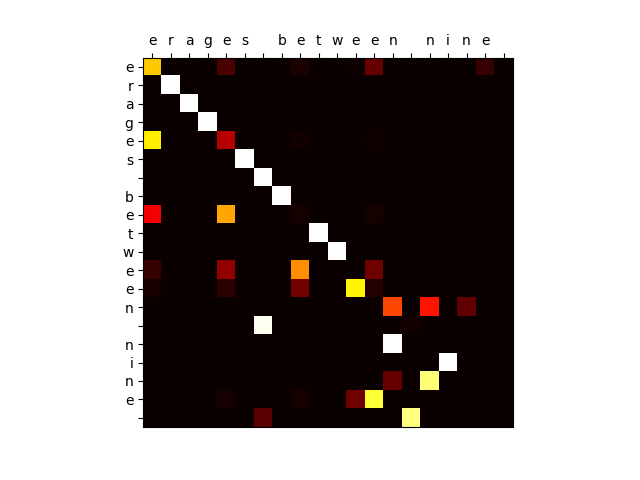
\includegraphics[width=0.7\textwidth]{attn_q2.png}
\caption{Layer-1 attention map for the input ``erages between nine '' (2-layer Transformer, BEFORE task).
Rows are query positions; columns are key positions. Brighter = higher attention weight.}
\label{fig:q2}
\end{figure}

The attention map shows a clear lower-triangular pattern: each position primarily attends to earlier positions that contain the same character (e.g., the second `e' attends back to the first `e', and the second `n' attends back to the first `n'). This is exactly what we expect---the model uses attention to count how many times the same letter has appeared before, and positional encoding lets it restrict attention to only previous positions.

\section*{Q3: More Transformer Layers}

With 3--4 Transformer layers, the first layer still shows the interpretable pattern from Q2 (attending to prior occurrences of the same character). However, deeper layers produce much sparser or more diffuse attention maps that do not obviously correspond to same-character matching. This is expected: once the first layer encodes occurrence counts into the hidden representations, later layers no longer need to look back at raw characters---they refine the already-encoded features, so their attention patterns become less directly interpretable.

\end{document}
